\documentclass[sigconf]{acmart}
\usepackage{listings}
\usepackage{algorithm2e}
\settopmatter{printacmref=false} % Removes citation information below abstract
\renewcommand\footnotetextcopyrightpermission[1]{} % removes footnote with conference information in first column
\pagestyle{plain} % removes running headers

\begin{document}
\title{Word Suggestion Research Project Report}

\author{Ryan Wickman}
\affiliation{%
  \institution{University of Memphis}
  \streetaddress{3720 Alumni Ave}
  \city{Memphis}
  \state{Tennessee}
  \postcode{38152}}
  \email{rwickman@memphis.edu}

\author{Jordan Nichols}
\affiliation{%
  \institution{University of Memphis}
  \streetaddress{3720 Alumni Ave}
  \city{Memphis}
  \state{Tennessee}
  \postcode{38152}}
  \email{jnchols7@memphis.edu}

\maketitle

\section{Introduction}
In this section we will give a brief overview on the problem and approach of this project.
\subsection{Problem}
The problem of this project was to suggestion a word to user based upon the previous sequence of words they have entered. The challenges of this project included making the model behavior more personalized, learning a language model (e.g., n-gram) from a large collection of documentations (e.g., Wikipedia), and having a it highly engineered for real-time response.
\subsection{Approach}
In our approach to this problem we decided to focus on the language model first to gain better insight on how it works, then go about the research aspect. For the word suggestion model we used an RNN, with a the a word-embedding layer, Long Short-Term Memory (LSTM) layer, and a dense layer.

Then, this was improved upon by finding similar users by computing their similarity score and using their trained word suggestion model to provide suggestions for the user's sequence. We utilized Locality-Sensitive Hashing (LSH)/Minhashing to improve the real-time performance of this computation.

\section{Implementing the Word Suggestion model}
In this section, we provide how we went about implementing the word suggestion model. This is done through exploring the details of preprocessing data, building the model, training the model, and input into the model.
\subsection{Preprocessing data}
The training data was extracted from a dataset of dialogue of movies. This was chosen because it would assist the model by simulating a continuous conversation. The word suggestion model could then be initially trained on this data and thus provide a good base model for the user. For example, imagine someone said to the user, “Hello, how are you?”. The response should be “Good” or something similar. If instead the model was not trained in this way, it would give the same prediction every time the user hasn’t typed in anything yet, because it would be making predictions on the empty string. 

So, before being provided as training data into the model, the dialogue data needed to be cleaned. First each word was converted to lowercase. This was done so the space of words it needed to learn would be reduced. Second, removed all extra whitespace from the data. This included before and after each line of dialogue as well as if more than one space appeared between any words. Third, removed/replaced most non alphabet characters. We utilized Python’s re module to use RegEx for this: \lstinline{re.sub("[^a-z\'$% ]", "", text)}. This line will replace everything that is not in that list of characters with an empty character. Fourth, concatenated all the lines of dialogue to simulate a continuous conversation. Fifth, created a word to ID and ID to word dictionary that has mapping of each word to a unique ID and vice versa. Sixth, transformed each word in the dialogue text to unique ID equivalent. This was done because it is required for the model and typically allows for smaller representation of the data.
\subsection{Building the Model}
Keras, which is a high-level library built on top of TensorFlow, was utilized to quickly create the network architecture of our word suggestion model. The architecture can be broken down into three layers. The first layer was an Embedding layer. This layer will take in the input sequence and map each unique ID to a new vector representation. This new vector representation is learned through training the model. It will update the vectors such that words that have similarity, such as synonyms or same subject area, will be put close together, while words that have lower correlation will be separated by a farther distance. This will provide some semantical understanding for the future layers. It’s input length was min(max sequence length, 40), the embedding dimension was 256, and the vocab size was 10,000. The second layer was an LSTM layer. This is the recurrent neural network (RNN) layer that will learn the relationship between sequences of words and will remember long dependencies between them. This was initialized with 1024 units. The third layer was a dense layer, which will transform the output of the LSTM layer into a probability distribution of the possible classes. This was initialized with 10,000 units, the same as the input vocab size, and uses the SoftMax activation function. Furthermore, while more complex architectures do exist, we kept it simple since it would suffice for our goal.

An Adam optimizer and a metric of Categorical Accuracy was use for the compilation, or configurations for training, of the model. The architecture can be viewed in Figure 1.
\begin{figure}[h]
    \centering
    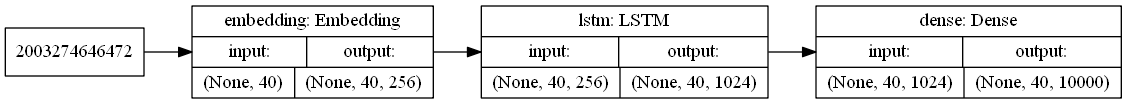
\includegraphics[width=\linewidth, scale=1.5]{figures/model.png}
    \caption{A visual representation of the word suggestion architecture.}
\end{figure}

\subsection{Training the Model}
When we first started training the model, we found the entire training set could not be loaded into memory. So instead of trying to fit on the entire dataset at once, a training generator was used\cite{lstmkeras}. This allows for the model to be trained on dynamic variable batch sizes and only load a subset of the dataset in memory at a time. At first, the model was only trained on a fixed sequence length. This made it difficult for it to make predictions on sequences of words that were not of this same fixed length. So, the generator was altered to produce random sequences of words, from 2 to the max sequence length for each training batch. This then increased the predictability on different sequence lengths. However, since variable sequence lengths were used, they had to be padded with 0’s to fit the input sequence length. 

The model was trained on 60 epochs, approximately 39 steps per epoch, and each batch size was of length 10. The results of the training were a loss value of 0.2381 and categorical accuracy of 95.11\lstinline{%}. The model has not been tested on a validation set. The reasoning for this is because we were not too concerned with overfitting the model since it should be fit uniquely to each user, rather than trying to be generalized for multiple people to use.
\pagestyle{plain} % removes running headers
\subsection{Input into the Model}
There are a few steps involved when providing input for the model for it to make a prediction. First, the input is cleaned, as discussed earlier. Second, words that were not initially trained in the model need to be filtered out. If this step was not done, it may cause an error when trying to make predictions on sequences that contain unforeseen IDs. This is due to the model having a limited vocab size. For example, if the word to ID dictionary length is equal to the vocab size, then any additional word mappings would produce an index greater than the capacity of the input for the model. This would throw an error. Of course, unforeseen words could be allowed until the upper limit has been reached, but that is beyond the scope of this project. Third, each word in the input is converted to a unique ID. Fourth, predict the next word in the sequence using the trained model. This is where the transformed input text is processed through the model, and the output would be a normalized probability distribution vector with dimensions 10,000 x 1. Each element in this vector corresponds to a probability of the word appearing next in the sequence, where its index corresponds to its ID. Fifth, the IDs are transformed back into their mapped word using the ID to word dictionary and sorted by likelihood of being the next word. An example of this is given in Figure 2.
\begin{figure}[h]
    \centering
    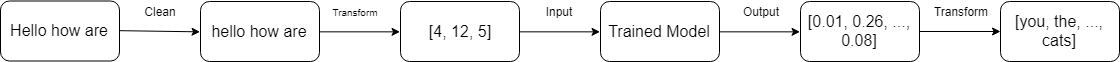
\includegraphics[width=\linewidth]{figures/Input_to_Model.png}
    \caption{An example of the steps that occurs when using the model to make a prediction on a sequence of words.}
\end{figure}

\section{Research on Improving the Other Models}
In this section, we present the design rationale of our approach to improving the model, how we then built and trained additional models, provide the algorithm, and explain a demo we built for this project.
\subsection{Design Rationale}
\textit{1) Personalize: }
We needed to improve the base language prediction model by making it more personalized. One thing that most word suggestion models already do is train on what the user has previously entered, so we kept this in the approach. However, to extend this, the solution we came up with is to find similar users and use their trained model for some suggestions. If the user selects a word that was suggested from a similar user’s model, the user’s model can be trained on a subset of that similar user’s dataset (e.g., song lyrics, a part of a conversation, etc.). This will allow for the user’s model to be trained on a larger input space, that has correlation to the user, and to have more verbose suggestions.

\textit{2) Similarity Metric: }
A similarity metric is required so that the user’s input thus far can be compared to a subset of a of a similar user’s dataset. The traditional approach to this would be to use Jaccard similarity. However, this is not efficient since the user will typically only enter a few words while the subset of data it is compared to can be rather large (e.g., greater than 100 words). Due to this, the intersection length between the user input and subset of data is rather small for most datasets while the union length is large. This will produce rather low similarity scores overall. So, to fix this issue, instead containment similarity can be applied, shown in Figure 3. Q is a query or in our case what the user as entered so far and X is some other dataset of words. The denominator is only the length of a query and not the union of two sets. This is essentially a normalized intersection that tends to have bias on the side of the user. Thus, allowing to find other users that use the same words as the user. This is used in LSH Ensemble.
\begin{figure}[h]
    \centering
    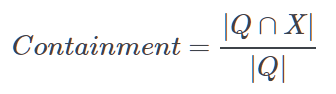
\includegraphics[width=0.5\linewidth]{figures/Containment_EQ.png}
    \caption{Containment Similarity.}
\end{figure}

\textit{3) Real-time Performance: }
The word suggestions should be given to the user in real-time. However, finding all similar users each time a new word is entered can take a long time. Instead, an approximation of this would be well suited. Through using MinHash and Locality Locality-Sensitive Hashing (LSH) we can reduce the overall time complexity and with respectable results. Specifically, Ensemble LSH will be applied because it uses containment similarity. More information about this can be found in the paper \textit{LSH Ensemble: Internet-Scale Domain Search}\cite{lshensemble}.

\subsection{Build and Train the Models}
First, two additional word suggestions models were trained to act as users for the purpose of experimentation. They use the same network architecture as the previous word suggestion model and are trained similarly. Albeit, one was trained on a dataset of song lyrics, while the other was trained on a dataset of movie quotes.

Next, I utilized the datasketch library to implement the approximate similarity models. Each subset of the dataset had its own MinHash (e.g., each song or movie). This was done through creating set of unique words from each subset then using MinHash with 128 permutation. Finally, they were used to initialize the LSH Ensemble model, which was configured with a containment threshold of 60\lstinline{%}. This specific threshold was used solely on empirical results, further study would be required to fine tune this number.

\subsection{Algorithm}

\begin{algorithm}
    \SetAlgoLined
    \KwResult{Word suggestions for the user}
    U = User\;
    P = All Other Users (or a subset of All Other Users)\;
    containment\_threshold = 0.60\;
     \If{user enters a new word}{
       word\_suggestions = []\;
      add U's model word suggestions to word\_suggestions\;
         \ForEach{p in P}{
           \ForEach{subset in p's dataset}{ 
              similarity\_score = containment similarity between U's entire entered sequence and subset\;
              \If{\lstinline{similarity_score >= containment_threshold}}{
                  p\_suggestions = p's model's predictions on U's entered sequence\;
                  add p\_suggestions to word\_suggestions\;
                  break\;
              }
          }
         }
         return word\_suggestions to U\;
         wait for U to pick or enter a new word\;
         Update U’s model with the sequence of words that U entered\;
         \If{U uses a word suggestion from a model in P}{
            Update U’s model by training on the subset of data associated with model in P\;
         }
     }
     \caption{Find similar users, create suggestions, and update the user's word suggestion model}
\end{algorithm}

\subsection{Demo}
A simple web interface was built to illustrate an application of this. The front-end was implemented using native HTML, CSS, and JavaScript. Then, to communicate between the front-end and the backend model, a WebSocket was set up. First, the front-end will send what the user has currently in the text-box, initially this is just an empty string. Second, the back-end receives this string and will undergo the necessary steps described above to get the word suggestions for the user. Third, the back-end will send the top 5 suggestions to the front-end. Fourth, the front-end will update the suggestions list with the newly predicted words.  This and the rests of the source code can be found here: https://github.com/rwickman/Word-Suggestion.

\section{Final Thoughts}
In this section we describe what adjustments could be made to the algorithm and what could be refactored and optimized in the implementation.
\subsection{Algorithm Adjustments}
The algorithm could be adjusted to consider the likelihood of two users being similar. This could be used to limit the number of users it has to compare. This could be represented as a symmetric matrix that gives the probability of two users beings similar. However, if instead this was a global matrix (i.e., used by multiple users) it may not make sense to make it symmetric, as it inherently would not be. This is because containment similarity is asymmetric and because it only considers what the user entered at a particular time rather than that user’s entire dataset of conversations. Therefore, an asymmetric matrix would be required instead. Some sort of centralized database would be required to maintain this type of matrix. 

Furthermore, as time goes on, there may be more obvious similarity relationships between users (i.e., two users may be more likely to be similar). This can be utilized to reduce the overall time required to find a certain number of similar users. 

The update step could be adjusted to improve real-time response and not waste a lot of the user’s device resources while in use. This could potentially be done through updating only when the user enters in a sequence rather than one word, updating only when the user is not actively using the word suggestion application, or done in a separate thread. The best approach may be application or device oriented.

\subsection{Refactoring and Optimizing Implementation}
There is a lot of optimizing and a bit of code refactoring that would need to be done if this was used in a production tool/application. This includes using the same generator for each dataset, using threading for predictions, using an API for similar user’s word suggestions model instead of loading and predicting locally, using an API for the similarity score computations, saving results from previous similarity score computations for reuse, fine tuning the amount of users the similarity metric is computed for, and a more that may be causing slower response time. Furthermore, if we had more time, we would have implemented LSH Ensemble ourselves. The library we were using had a lot of weird bugs \lstinline{(e.g., 64% threshold not working but 75% and 60% works)}. 

Another consideration is altering the word suggestion model to use a more complex model that would be able to learn more in depth information and find a good amount. Also, finding an efficient number of Epochs to train during the update step.


\bibliographystyle{ACM-Reference-Format}
\bibliography{ref}
\pagestyle{plain} % removes running headers
\end{document}